\section{What is the relationship between a pointer and an array (or string)?}
\begin{itemize}
    \item Arrays in C are sequential data items stored in some direction in memory.
    \item The address is as the array, is the same as the address of the first item in the array.
    \item The name of the array is also the address of the array.
    \item Let's see how strings are used in C.
\end{itemize}

\subsection{C strings}
\begin{itemize}
    \item In C strings are just arrays of characters.
    \item C treats the null character \mintinline{c}{'\0'} as the string's terminator.
        \begin{minted}[autogobble]{c}
            #include <stdio.h>
            int main() {
                char str1[] = "Hello world";
                printf("%s %c %d %d\n", str1, str1[0], &str1, &str1[0], str1);
                return 0;
            }
            /* Output:
            Hello world H 312473588 312473588
            */
        \end{minted}

    \item Note that the string is stored in location 312473588 in RAM. When printing the address of the first element of the array and the address of the array we get exactly the same location.
\end{itemize}

\subsection{Continuation}
\begin{itemize}
    \item The address of an array is the same as the address of the first element in the array because it is where the array begins. The name of the array is mapped to the address of the array by the compiler, thus we can say that the name of the array is the location of the array and the location of the array is the location of the first member of the array.
    \item Array is a location in memory, thus an array is a pointer. However all thought an array is a pointer, it is not handled the same as a pointer in C. A pointer variable needs to be handled differently than an array, although behind the scenes an array is a pointer.
\end{itemize}

%%%%%%%%%%%%%%%%%%%%%%%%%%%%%%%%%%%%%%%%%%%%%%%%%%%%%%
\section{Arrays, addresses, and pointers}
\begin{itemize}
    \item Notice the following code and it's output:
        \begin{minted}[autogobble]{c}
            #include <stdio.h>
            int main() {
                char str1[] = "Hello"; // Array
                char *str2 = "Goodbye"; // Pointer
                printf("%u %u %s\n", &str1, str1, str1);
                printf("%u %u %s\n", &str2, str2, str2);
                return 0;
            }
            /*
            Output:
            3558866218 3558866218 Hello
            3558866208 686526464 Goodbye
            */
        \end{minted}
    
    \item Notice that when outputing the array str1's address and the array itself we get the same one, this is because the array is the pointer to the string "Hello". Notice that when outputing the array str2's address we get a different address than the str2 variable, that is because when we get the address of a pointer, a pointer has a location in memory, and the value of a pointer references the string, the pointer has a location in memory, different to the array pointer, the pointer is not the array in this case, the pointer is a separate variable that makes reference to the array as it's value.
    \item Thus the second direction is different because we are printing the pointer address and the array address, which is not the same.
    \item An array variable such as str1 is an address, it is it's own address, the array variable is the address of the array.
    \item But a pointer variable is not an array, it is a variable that stores the address of the array. The pointer variable itself is stored in one address, and the array is stored in another.
    \item Think of the example we gave earlier, the giant lot of warehouses that are labled and we need to go to warehouse 13.
        \begin{figure}[H]
            \centering
            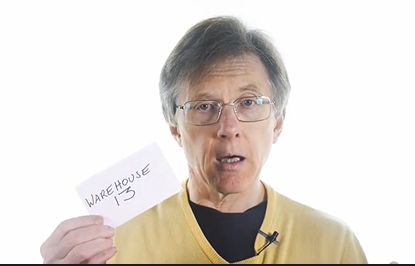
\includegraphics[width=\width\textwidth]{./figs/20220610151106.png}
            %\caption{}
        \end{figure}
    
    \item The card is like a pointer variable, it is not the location, it contains the value of the location of the warehouse. The warehouse is like the array, it is not just a reference to the location, it is the location. The pointer is like the card containing the text "warehouse 13" the card is not the location, it contains the location that we need to go to, the card is not the warehouse 13.
        \begin{figure}[H]
            \centering
            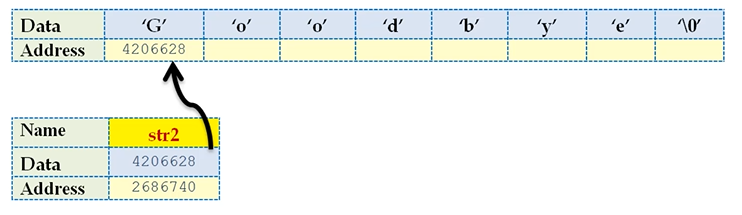
\includegraphics[width=\width\textwidth]{./figs/20220610151411.png}
            %\caption{}
        \end{figure}
    
    \item Let's try out another example:
        \begin{minted}[autogobble]{c}
            #include <stdio.h>
            int main() {
                char str1[] = "Hello"; // Array
                char *str2 = str1; // Pointer
                printf("%u %u %s\n", &str1, str1, str1);
                printf("%u %u %s\n", &str2, str2, str2);
                return 0;
            }
            /*
            Output:
            3911186266 3911186266 Hello
            3911186256 3911186266 Hello
            */
        \end{minted}
    
    \item Notice that get the different numbers in the second printing because now the pointer variable is pointing to the array. See how each of them are different? One is the reference to the location of the array and the other is the array.
\end{itemize}

%%%%%%%%%%%%%%%%%%%%%%%%%%%%%%%%%%%%%%%%%%%%%%%%%%%%%%
\section{Multiple indirection}
\begin{itemize}
    \item A pointer can also point to another pointer.
    \item For exapmle: \mintinline{c}{int **ppi;}
    \item When we use a pointer to access data at an address we call it indirection or dereferencing.
    \item Using a pointer to access data from another pointer is called multiple indirection. Because it requires more than one step.
    \item Why would we ever need multiple indirection?
        \begin{itemize}
            \item We might have a list of lists, that are accessed using pointer to pointer.
        \end{itemize}
\end{itemize}

%%%%%%%%%%%%%%%%%%%%%%%%%%%%%%%%%%%%%%%%%%%%%%%%%%%%%%
\section{Multiple indirection with integers}
\begin{minted}[autogobble]{c}
    #include <stdio.h>
    #define LENGTH 3
    int data[LENGTH]; // array of integers.
    int main(int argc, char **argv) {
        int *pi; // pointer to an int.
        int **ppi; // pointer to pointer to int.
        printf("multiple indirection example\n");
        // initialize our integer array.
        for (int i = 0; i < LENGTH; i++) {
            data[i] = i;
        }
        for (int i = 0; i < LENGTH; i++) {
            printf("%d\n", data[i]);
        }
        /*
        A: simple pointer to a pointer to an integer.
        */
        pi = data; // the address of data is assigned to pi.
        ppi = &pi; // the ppi points to the pointer pi.
        for (int i = 0; i < LENGTH; i++) {
            printf("\nLoop[%d] array address is %u\n", i, data);
            printf("item pointed to by pi is %d\n", *pi);
            printf("item pointed to by ppi is %u\n", *ppi);
            printf("item pointed to by double indirection of ppi is %d\n\n", **ppi);
            printf("The address of pi is %u\n\tand the value of pi (what it points to) is %u\n\n", &pi, ppi);
            pi += 1;
        }
        return 0;
    }
    /*
    multiple indirection example
    0
    1
    2

    Loop[0] array address is 341364800
    item pointed to by pi is 0
    item pointed to by ppi is 341364800
    item pointed to by double indirection of ppi is 0

    The address of pi is 727710864
            and the value of pi (what it points to) is 727710864


    Loop[1] array address is 341364800
    item pointed to by pi is 1
    item pointed to by ppi is 341364804
    item pointed to by double indirection of ppi is 1

    The address of pi is 727710864
            and the value of pi (what it points to) is 727710864


    Loop[2] array address is 341364800
    item pointed to by pi is 2
    item pointed to by ppi is 341364808
    item pointed to by double indirection of ppi is 2

    The address of pi is 727710864
            and the value of pi (what it points to) is 727710864
    */
\end{minted}
\begin{itemize}
    \item Notice the above code.
    \item The area we are really interested in understanding is the for loop with the multiple indirection. Lets have a closer look:
        \begin{minted}[autogobble]{c}
            for (int i = 0; i < LENGTH; i++) {
        \end{minted}
        \begin{itemize}
            \item Iterating from i=0 to the length of the array.
        \end{itemize}
        \begin{minted}[autogobble]{c}            
            printf("\nLoop[%d] array address is %u\n", i, data);
        \end{minted}
        \begin{itemize}
            \item This statement will print the index which we are using right now. And the address of the array data.
        \end{itemize}
        \begin{minted}[autogobble]{c}
            printf("item pointed to by pi is %d\n", *pi);
        \end{minted}
        \begin{itemize}
            \item This statement is used to print the value of the pointer pi.
        \end{itemize}
        \begin{minted}[autogobble]{c}
            printf("item pointed to by ppi is %u\n", *ppi);
        \end{minted}
        \begin{itemize}
            \item This statement is used to print the value of ppi, which is another pointer, thus the value being printed is the decimal form location of the other pointer in memory.
        \end{itemize}
        \begin{minted}[autogobble]{c}
            printf("item pointed to by double indirection of ppi is %d\n\n", **ppi);
        \end{minted}
        \begin{itemize}
            \item This statement is using double indiretion to access the data pointed to by the double pointer. 
                \begin{figure}[H]
                    \centering
                    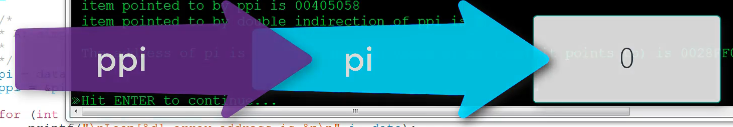
\includegraphics[width=\width\textwidth]{./figs/20220610222400.png}
                    %\caption{}
                \end{figure}
            
            \item Notice the \mintinline{c}{**ppi}, the double asterisk is to dereference twice. Get the value of the value of the pointer.
        \end{itemize}
        \begin{minted}[autogobble]{c}
            printf("The address of pi is %u\n\tand the value of pi (what it points to) is %u\n\n", &pi, ppi);
        \end{minted}
        \begin{itemize}
            \item This statement is used to print the address of the pointer pi and also to print the pointer ppi, ppi is pointing to the address of pi, thus the address will always be the same in this program.
        \end{itemize}
        \begin{minted}[autogobble]{c}
            pi += 1;
            }
        \end{minted}
        \begin{itemize}
            \item pi is a pointer and it will be incremented by 1, since it is an int pointer it will be incremented by the sizeof one int. This is called pointer arithmetic.
        \end{itemize}
\end{itemize}

%%%%%%%%%%%%%%%%%%%%%%%%%%%%%%%%%%%%%%%%%%%%%%%%%%%%%%
\section{Multiple indirection with strings}
\begin{minted}[autogobble]{c}
    #include <stdio.h>
    #define LENGTH 3
    char *words[LENGTH]; // array of char.
    int main(int argc, char **argv) {
        char *pc; // pointer to an char.
        char **ppc; // pointer to pointer to char.
        printf("multiple indirection example\n");
        // initialize our integer array.
        words[0] = "zero";
        words[1] = "one";
        words[2] = "two";
        for (int i = 0; i < LENGTH; i++) {
            printf("%s\n", words[i]);
        }
        /*
        B: simple pointer to an array of strings.
            The same as a pointer to a pointer to a character.
        */
        printf("\nNow print the chars of each string...\n");
        ppc = words; // ppc is pointing to the array location of words.
        for (int i = 0; i < LENGTH; i++) {
            ppc = words + i; // initialize the pointer to a pointer to a character
            pc = *ppc; // loop over each string.
            while (*pc != 0) {
                printf("%c ", *pc); // process each character in a string.
                pc += 1; // print out each character of the string individual.
            }
            printf("\n");
        }
        return 0;
    }
    /* Output:
    multiple indirection example
    zero
    one
    two

    Now print the chars of each string...
    z e r o
    o n e
    t w o
    */
\end{minted}

%%%%%%%%%%%%%%%%%%%%%%%%%%%%%%%%%%%%%%%%%%%%%%%%%%%%%%
\section{Indirection and commandline args}
\begin{itemize}
    \item As you know C programs accept command line arguments, we send these to the main function using the arguments argc and argv. The argv is a pointer to a pointer to a char.
        \begin{minted}[autogobble]{c}
            int main(int argc, char **argv) {
                ...
            }
        \end{minted}
    
    \item The argc is the amount of arguments passed to the program, the argv variable is a pointer to a pointer of chars, which is an array of strings.
    \item Let's see an example:
        \begin{minted}[autogobble]{c}
            #include <stdio.h>
            int main(int argc, char **argv) {
                for (int i = 0; i < argc; i++) {
                    printf("arg %d is %s\n", i, argv[i]);
                }
                printf("\n\n");
                for (int i = 0; i < argc; i++) {
                    printf("arg %d is %s\n", i, *argv);
                    argv++;
                }
                return (0);
            }
            /* Output:
            arg 0 is a
            arg 1 is hello
            arg 2 is this
            arg 3 is an
            arg 4 is argv
            arg 5 is argument
            arg 6 is setence


            arg 0 is a
            arg 1 is hello
            arg 2 is this
            arg 3 is an
            arg 4 is argv
            arg 5 is argument
            arg 6 is setence
            */
        \end{minted}
\end{itemize}

%%%%%%%%%%%%%%%%%%%%%%%%%%%%%%%%%%%%%%%%%%%%%%%%%%%%%%
\section{Generic pointers}
\begin{itemize}
    \item Sometimes we have a function that needs to perform an operation using several inputs. If the inputs are double, float, int or long does not matter, this case you would be inclined to write the same function for all the data types, but you would not be adviced to not duplicate code. We can write just one funtion that takes in a generic pointer instead.
    \item A generic pointer is a pointer to void. To use it you must cast it into a data type.
    \item This is useful since it gives us more liberty and allows us to not repeat code.
\end{itemize}

\subsection{Example}
\begin{minted}[autogobble]{c}
    #include <stdio.h>

    #define LENGTH 3
    int data[LENGTH];
    char *words[LENGTH];

    int main(int argc, char **argv) {
        void *gp;
        printf("generic pointer example\n");

        // initialize out integer array.
        for (int i = 0; i < LENGTH; i++) {
            data[i] = i;
        }
        for (int i = 0; i < LENGTH; i++) {
            printf("%d\n", data[i]);
        }
        // initialize our string array.
        words[0] = "zero";
        words[1] = "one";
        words[2] = "two";
        for (int i = 0; i < LENGTH; i++) {
            printf("%s\n", words[i]);
        }
        // example of a generic pointer.
        gp = data;
        printf("\ndata array address is %p\n", gp);
        // cast to int *. then dereference.
        printf("item pointed to by gp is %d\n", *(int*)gp);
        gp = (int*)gp + 1; // casting to a pointer to int. add 1.
        printf("item pointer to by gp is now %d\n", *(int*)gp);
        // now using the pointer to point to a string.
        gp = words;
        printf("\nwords arra address is %p", gp);
        // cast to a char ** and then dereference the pointer.
        printf("item pointed to by gp is %s\n", *(char**)gp);
        gp = (char**)gp + 1; // dereference and now add one
        printf("item pointed to by gp is now %s", *(char**)gp);
        return (0);
    }
    /* Output:
    0
    1
    2
    zero
    one
    two

    data array address is 00007ff695f6d040
    item pointed to by gp is 0
    item pointer to by gp is now 1

    words arra address is 00007ff695f6d050item pointed to by gp is zero
    item pointed to by gp is now one
    */
\end{minted}

%%%%%%%%%%%%%%%%%%%%%%%%%%%%%%%%%%%%%%%%%%%%%%%%%%%%%%
\section{Allocating memory}
\begin{itemize}
    \item When we created arrays in the previous examples they were created we assigned a string. The memory is allocated for these bytes of data. But sometimes we don't know how much memory to allocate at compile time, we need the ability to allocate memory at run time.
    \item We can handle memory allocation using the malloc function.
    \item The malloc function returns a pointer to void, it allocates the memory we need at run time, thus we can request and free memory at run time as needed.
    \item The malloc function allocates memory in an area called the heap, normal arrays are allocated on the stack.
\end{itemize}

\subsection{Example}
\begin{minted}[autogobble]{c}
    #include <stdio.h>
    #include <string.h>
    #include <malloc.h>

    #define MAXSTRLEN 100

    char *string_function(char *astring) {
        char *s;
        s = (char*)malloc(MAXSTRLEN);
        s[0] = 0; // initialize first char to null.
        strcat(s, "Hello ");
        strcat(s, astring);
        strcat(s, "\n");
        return s;
    }

    int main(int argc, char **argv){
        printf(string_function("Fred"));
        printf(string_function("Gussie Fink-Nottle"));
        return 0;
    }

    /* Output:
    Hello Fred
    Hello Gussie Fink-Nottle
    */
\end{minted}

\subsection{Conclutions}
\begin{itemize}
    \item The implementation above has some problem, namely that there fould be a string passed in that is larger than 100 bytes, and therefore we can have a buffer overflow problem. Also all space allocated in the heap needs to be explicitly freed, this is a concept we will cover later. 
    \item Thus the above implementation is flawed.
\end{itemize}

%%%%%%%%%%%%%%%%%%%%%%%%%%%%%%%%%%%%%%%%%%%%%%%%%%%%%%
\section{Malloc and sizeof}
\begin{itemize}
    \item Let's see how we can allocate just the right amount of memory:
        \begin{minted}[autogobble]{c}
            #include <stdio.h>
            #include <stdlib.h>
            #include <string.h>

            int main() {
                char *s;
                int stringsize;
                stringsize = sizeof("hello"); // sizeof operator calculates the size of the data.
                printf("size of 'hello' is %d\n", stringsize);

                s = (char*)malloc(stringsize);
                // if malloc returns null then there was an error and we must terminate the program.
                if (s == NULL) {
                    printf("malloc failed.");
                    exit(0);
                }
                // now copy the stirng into the newly allocated string.
                strncpy(s, "hello", stringsize);

                // and change the first character (just to show we can)
                printf("s is %s\n", s);
                s[0] = 'c';
                printf("s is now %s\n", s);
                return (0);
            }
            /* Output:
            size of 'hello' is 6
            s is hello
            s is now cello
            */
        \end{minted}
\end{itemize}

%%%%%%%%%%%%%%%%%%%%%%%%%%%%%%%%%%%%%%%%%%%%%%%%%%%%%%
\section{Functions that cause errors or warnings}
\begin{itemize}
    \item Sometimes when using some functions, a warning will appear that will tell you that the function you are using is deprecated. There are sometimes reasons to still use them for example, to make the functions compatible with any C compiler. 
    \item In many cases the best option will be to use the recomended function. Or you could define the constant \mintinline{c}{_CRT_SECURE_NO_WARNINGS} to turn off the deprecateion warnings.
    \item By placing the constant:
        \begin{minted}[autogobble]{c}
            #define _CRT_SECURE_NO_WARNINGS
        \end{minted}
    
    \item The compiler should stop pestering you about the deprecation status of the functions you use.
\end{itemize}

%%%%%%%%%%%%%%%%%%%%%%%%%%%%%%%%%%%%%%%%%%%%%%%%%%%%%%
\section{calloc}
\begin{itemize}
    \item There is a function called calloc that is similar to malloc. The calloc function performs everything the malloc function would but it also performs the aditional step of clearing the memory with nulls.
    \item Uninitialized memory contains junk. You could allocate memory and the memory you allocate can contain anything, thus it is prone to errors and bugs. 
    \item If you allocate memory with calloc the memory is allocated and cleared out with all 0s.
    \item If you are careful and always initialize all the memory after using malloc, then by all means use malloc. Otherwise use calloc.
\end{itemize}

\subsection{Parameter differences between calloc and malloc}
\begin{itemize}
    \item malloc just takes in the amount of memory in bytes to be allocated.
        \begin{minted}[autogobble]{c}
            s = (char*)malloc(6);
        \end{minted}
    \item calloc takes in two parameters, first the amount of elements to be allocated, then the size of each element.
        \begin{minted}[autogobble]{c}
            s = (char*)calloc(6, sizeof(char)); // total space allocated 6*1.
        \end{minted}
    
    \item Basically the calloc function will mutliply the amount of elements with the space required by each element.
    \item Notice the following example, we allocate memory and print the data contained within that space. Look that random numbers are thrown. Then using calloc, it is always 0s.
        \begin{minted}[autogobble]{c}
            #include <stdio.h>
            #include <stdlib.h>
            #include <string.h>

            int main() {
                char *s;
                int *p;
                s = (char*)malloc(6);
                for (int i = 0; i < 6; i++) { printf("s[%d]=%d\n", i, s[i]); }
                printf("\n");

                s = (char*)calloc(6, sizeof(char));
                for (int i = 0; i < 6; i++) { printf("s[%d]=%d\n", i, s[i]); }
                free(s);
                printf("\n");

                p = (int*)calloc(6, sizeof(int));
                for (int i = 0; i < 6; i++) { printf("p[%d]=%d\n", i, p[i]); }
                free(p);
                return (0);
            }
            /* Output:
            s[0]=16
            s[1]=104
            s[2]=119
            s[3]=12
            s[4]=-108
            s[5]=1

            s[0]=0
            s[1]=0
            s[2]=0
            s[3]=0
            s[4]=0
            s[5]=0

            p[0]=0
            p[1]=0
            p[2]=0
            p[3]=0
            p[4]=0
            p[5]=0
            */
        \end{minted}
\end{itemize}

\subsection{Null pointers}
\begin{itemize}
    \item Both calloc and malloc will return NULL pointer if the allocation fails. A null pointer is a pointer whose value is 0. By convention, a pointer with the value 0 is a pointer that does not contain a valid address.
    \item We can test for a null pointer by comparing it to the NULL constant.
\end{itemize}

%%%%%%%%%%%%%%%%%%%%%%%%%%%%%%%%%%%%%%%%%%%%%%%%%%%%%%
\section{free}
\begin{itemize}
    \item Once memory is allocated it is no longer available to the rest of your program. 
    \item So you can run out of memory if you don't free it.
    \item This only applies to memory inside the heap, the stack memory is managed by the compiler.
    \item Keeping memory allocated is waste. 
    \item Memory allocated but not used is called a memory leak. This can be a real problem for devices that don't have much memory, such as embeded devices or even device controlers.
    \item When the memory is no longer need you must free it. 
    \item To free allocated memory you just need to call free with the pointer you used to allocate.
    \item In the previous example we used free:
        \begin{minted}[autogobble]{c}
            free(s); // the only parameter is the pointer to the allocated data.
        \end{minted}
    
    \item If you call free on a variable that was never allocated or try to use allocated memory after you call free then your program can go horribly wrong.
\end{itemize}

%%%%%%%%%%%%%%%%%%%%%%%%%%%%%%%%%%%%%%%%%%%%%%%%%%%%%%
\section{realloc}
\begin{itemize}
    \item To change the size of allocated memory you might use the realloc function.
    \item Suppose we've allocated enough space for the characters 'hello'. And now we require enough space for 'hello world', if we were to simply strcpy this new string into a buffer with just enough space to say 'hello' we will have a buffer overflow. And the resulting program will be unpredictable because we are accessing unreserved memory space.
        \begin{minted}[autogobble]{cpp}
            char *s;
            int i;

            i = sizeof("hello");
            s = (char*)malloc(i);
            strncpy(s, "hello world"); // buffer overflow
            printf("s is %s\n", s);

            strcat(s, " world"); // program crashes, buffer overflow.
            printf("s is now %s\n", s);
        \end{minted}

    \item Using realloc we can expand or shrink the size of allocated memory. The solution is the following:
        \begin{minted}[autogobble]{cpp}
            #include <stdio.h>
            #include <stdlib.h>
            #include <string.h>

            int main() {
                char *s;
                int i;

                i = sizeof("hello");
                s = (char*)malloc(i);
                strncpy(s, "hello");
                printf("s is %s\n", s);

                realloc(s, 12);
                strcat(s, " world"); // program crashes, buffer overflow.
                printf("s is now %s\n", s);

                free(s);
                return (0);
            }
            /* Output:
            s is hello
            s is now hello world
            */
        \end{minted}
\end{itemize}

%%%%%%%%%%%%%%%%%%%%%%%%%%%%%%%%%%%%%%%%%%%%%%%%%%%%%%
\section{Pointer arithmetic}
\begin{itemize}
    \item When iterating arrays, weve advanced to the next element of the array using the \mintinline{cpp}{ptr += 1} statement, but the elements are variable in size, one element can be an int which occupies 4 bytes, adding 1 would not advance to the next element in this case. This is because dispite adding 1 conceptually doesnt land us in the next element. The compiler behind the scenes adds 1 times the sizeof the element to get the element.
    \item The compiler does this with pointers because the what is being pointed to only makes sense to advance it by the size of the elements of the array not by individual bytes.
        \begin{minted}[autogobble]{cpp}
            #include <stdio.h>
            #include <stdlib.h>
            #include <string.h>

            #define COUNT 4

            int main() {
                int *p;
                int a[COUNT];

                for (int i = 0; i < COUNT; i++) {
                    a[i] = i;
                }
                p = a;
                printf("Address of a is %p; value of p is %p [%d]; value pointed to by p is %d\n", a, p, p, *p);

                p = p + 1;
                printf("Address of a is %p; value of p is %p [%d]; value pointed to by p is %d\n", a, p, p, *p);

                p = p + 2;
                printf("Address of a is %p; value of p is %p [%d]; value pointed to by p is %d\n", a, p, p, *p);

                p = p + 1; // exceded the bounds of the array. Run time overflow.
                printf("Address of a is %p; value of p is %p [%d]; value pointed to by p is %d\n", a, p, p, *p);
                
                return (0);
            }
            /* Output:
            Address of a is 00000055a25ffa10; value of p is 00000055a25ffa10 [-1570768368]; value pointed to by p is 0
            Address of a is 00000055a25ffa10; value of p is 00000055a25ffa14 [-1570768364]; value pointed to by p is 1
            Address of a is 00000055a25ffa10; value of p is 00000055a25ffa1c [-1570768356]; value pointed to by p is 3
            Address of a is 00000055a25ffa10; value of p is 00000055a25ffa20 [-1570768352]; value pointed to by p is -1570768352
            */
        \end{minted}
\end{itemize}

%%%%%%%%%%%%%%%%%%%%%%%%%%%%%%%%%%%%%%%%%%%%%%%%%%%%%%
\section{Calculating an array index}
\begin{itemize}
    \item As you saw, adding one to a pointer increases its value by the size in bytes of the data its pointing to. If its an array of ints the increments will take place in steps of 4, if its an array of chars it will take place in steps of 1.
        \begin{minted}[autogobble]{cpp}
            #include <stdio.h>
            #include <stdlib.h>
            #include <string.h>

            #define COUNT 4

            int main() {
                int *pa;
                float *pb;
                double *pc;
                long long int *pd;
                short int *pe; 
                long int *pf;

                int a[COUNT];
                float b[COUNT];
                double c[COUNT];
                long long int d[COUNT];
                short int e[COUNT];
                long int f[COUNT];

                printf("sizes are: int %d; float %d; double %d; long long int %d; short int %d; long int %d\n", sizeof(int),
                    sizeof(float), sizeof(double), sizeof(long long int), sizeof(short int), sizeof(long int));

                pa = a; pb = b; pc = c; pd = d; pe = e; pf = f;
                for (int i = 0; i < COUNT; i++) {
                    a[i] = b[i] = c[i] = d[i] = e[i] = f[i] = i;
                }

                pa += 1;
                pb += 1;
                pc += 1;
                pd += 1;
                pe += 1;
                pf += 1;

                printf("address of a is %p [%u]; value of pa is %p [%u]; value pointed to by pa is %d\n", a, a, pa, pa, *pa);
                printf("address of b is %p [%u]; value of pb is %p [%u]; value pointed to by pb is %f\n", b, b, pb, pb, *pb);
                printf("address of c is %p [%u]; value of pc is %p [%u]; value pointed to by pc is %f\n", c, c, pc, pc, *pc);
                printf("address of d is %p [%u]; value of pd is %p [%u]; value pointed to by pd is %lld\n", d, d, pd, pd, *pd);
                printf("address of e is %p [%u]; value of pe is %p [%u]; value pointed to by pe is %hd\n", e, e, pe, pe, *pe);
                printf("address of f is %p [%u]; value of pf is %p [%u]; value pointed to by pf is %ld\n", f, f, pf, pf, *pf);

                return 0;
            }
            /*
            Output:
            sizes are: int 4; float 4; double 8; long long int 8; short int 2; long int 4
            address of a is 000000f5afdff9a0 [2950691232]; value of pa is 000000f5afdff9a4 [2950691236]; value pointed to by pa is 1
            address of b is 000000f5afdff990 [2950691216]; value of pb is 000000f5afdff994 [2950691220]; value pointed to by pb is 1.000000 
            address of c is 000000f5afdff970 [2950691184]; value of pc is 000000f5afdff978 [2950691192]; value pointed to by pc is 1.000000
            address of d is 000000f5afdff950 [2950691152]; value of pd is 000000f5afdff958 [2950691160]; value pointed to by pd is 1        
            address of e is 000000f5afdff948 [2950691144]; value of pe is 000000f5afdff94a [2950691146]; value pointed to by pe is 1
            address of f is 000000f5afdff930 [2950691120]; value of pf is 000000f5afdff934 [2950691124]; value pointed to by pf is 1 
            */
        \end{minted}
    
    \item Notice that advancing the pointer by one is not always advancing it by one byte but advancing it by the size in bytes of each element in the arrays.
    \item Sometimes the data types are different sizes on different machines, for example on a PC the size of the long int is 4 and on a mac it is 8 bytes. This is why its better to have the \mintinline{cpp}{+= 1} notation since different systems can advance the pointers according to their specific sizes and we are not left with the problem of hardcoding the wrong data type size.
\end{itemize}

%%%%%%%%%%%%%%%%%%%%%%%%%%%%%%%%%%%%%%%%%%%%%%%%%%%%%%
\section{Pointers to structs}
\begin{itemize}
    \item Structs vary in size according to the order of their attributes.
    \item For example the following struct may take the size of the sum of its data types.
        \begin{minted}[autogobble]{cpp}
            typedef struct {
                int a; // 4 bytes
                int c; // 4 bytes
                double b; // 8 bytes
                long long int d; // 8 bytes
            }
            // 24 bytes in total?
        \end{minted}
    
    \item It maybe the case that the compiler determines the size of the struct to be 24, however the same struct with changed order of attributes will not be equivalent in size to the above struct:
        \begin{minted}[autogobble]{cpp}
            typedef struct {
                int a; // 4 bytes
                double b; // 8 bytes
                int c; // 4 bytes
                long long int d; // 8 bytes
            }
            // 24 bytes in total? Now its 32 bytes.
        \end{minted}
    
    \item Merely changing the order of attributes prompts the compiler to add padding space and the size may no longer be 24. So to be safe NEVER ASSUME THE SUM OF THE ATTRIBUTES OF A STRUCT IS ITS SIZE, use the sizeof operator instead. sizeof returns the correct value regardless of what the true space allocated ends up being.
    \item To understand why the C compiler does not use exactly the required space to allocate structs we must understand how the C compiler alligns the data in memory. This is the content of the next lecture.
\end{itemize}

%%%%%%%%%%%%%%%%%%%%%%%%%%%%%%%%%%%%%%%%%%%%%%%%%%%%%%
\section{Data type alignment}
\begin{itemize}
    \item Reordering the fields of a struct may lead to the compiler using more space than just the sum of the sizes of the attributes.
    \item The data types are being aligned in memory. To understand this we must imagine that struct memory is layed out int rows of 8 bytes. Like so:
        \begin{figure}[H]
            \centering
            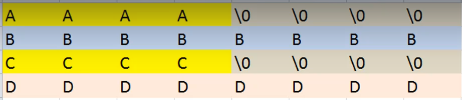
\includegraphics[width=\width\textwidth]{./figs/20220621193150.png}
            %\caption{}
        \end{figure}
    
    \item When we put an int first the 4 remaining bytes of the 8 byte row are used as padded to accomodate the next data types which is a double, this one will take the whole row. Then again an int with 4 bytes of padding and then finally the double. By placing the ints consecutively we are avoiding padding and instead of taking 32 bytes we take only 24 since we did not use padding:
        \begin{figure}[H]
            \centering
            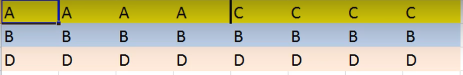
\includegraphics[width=\width\textwidth]{./figs/20220621193333.png}
            %\caption{}
        \end{figure}
\end{itemize}

%%%%%%%%%%%%%%%%%%%%%%%%%%%%%%%%%%%%%%%%%%%%%%%%%%%%%%
\section{Type alignment on boundaries}
\begin{itemize}
    \item Data types of a certain size are aligned at boundaries of that size.
    \item An int will be aligned at boundaries of 4 bytes, a double will be aligned at boundaries of 8 bytes. The take on knowing this is not to predict the size of the struct, but to understand that the size of a struct cannot be assumed. 
    \item Even if you manage to guess correctly using alignment and predicting the size, different machines have different sizes for the data types you are using. 
    \item In short, always always use sizeof because it is the only way to ensure the size of the struct in bytes is calculated correctly.
    \item The ways structs are stored in memory is unpredictable accross different arquitectures and systems.
    \item Even making an apparently trivial change such as rearranging the fields may alter the amount of memory it needs.
\end{itemize}

%%%%%%%%%%%%%%%%%%%%%%%%%%%%%%%%%%%%%%%%%%%%%%%%%%%%%%
\section{Type alignment and pointer arithmetic}
\begin{itemize}
    \item Never assume the size of data types. Especially when allocating memory. Instead of hardcoding the presuposed size, use the sizeof operator to calculate the amount of memory needed.
        \begin{minted}[autogobble]{cpp}
            #include <stdio.h>
            #include <stdlib.h>
            #include <string.h>

            typedef struct {
                int a; // 4 bytes
                int c; // 4 bytes
                double b; // 8 bytes
                long long int d; // 8 bytes
            } MYSTRUCT;

            #define COUNT 4

            int main() {
                MYSTRUCT *p, *q;
                void *v;
                printf("size of MYSTRUCT = %d\n", sizeof(MYSTRUCT));
                p = (MYSTRUCT*)calloc(COUNT, sizeof(MYSTRUCT));
                
                for (int i = 0; i < COUNT; i++) {
                    p[i].a = i;
                    p[i].b = 1000000000000.0 + i;
                    p[i].c = i * 20;
                    p[i].d = 4294967296 + i;
                }
                q = p;

                printf("[0] values:\na is %d\nb is %f\ncis %d\nd is%lld\n", q->a, q->b, q->c, q->d);
                printf("addresses:\na is %p\nb is %p\nc is %p\nd is %p\n", &q->a, &q->b, &q->c, &q->d);

                q = p + 1;

                printf("[1] values:\na is %d\nb is %f\ncis %d\nd is%lld\n", q->a, q->b, q->c, q->d);
                printf("addresses:\na is %p\nb is %p\nc is %p\nd is %p\n", &q->a, &q->b, &q->c, &q->d);

                v = p + 1;
                printf("struct at index 1\n");
                for (int i = 0; i < sizeof(MYSTRUCT) / sizeof(int); i++) {
                    printf("v[%d]=%d\n", i, ((int*)v)[i]);
                }
                
                return (0);
            }
            /*
            Output:
            size of MYSTRUCT = 24
            [0] values:
            a is 0
            b is 1000000000000.000000
            cis 0
            d is4294967296
            addresses:
            a is 0000025f4dda69a0
            b is 0000025f4dda69a8
            c is 0000025f4dda69a4
            d is 0000025f4dda69b0
            [1] values:
            a is 1
            b is 1000000000001.000000
            cis 20
            d is4294967297
            addresses:
            a is 0000025f4dda69b8
            b is 0000025f4dda69c0
            c is 0000025f4dda69bc
            d is 0000025f4dda69c8
            struct at index 1
            v[0]=1
            v[1]=20
            v[2]=-1577050112
            v[3]=1114446484
            v[4]=1
            v[5]=1
            */
        \end{minted}
    
    \item See the padding space and the locations of attributes in the structs. You can see the padding explicitly by checking the pointer addresses.
\end{itemize}